L'équipe de recherche et de développement du projet est composée de quatre élèves étudiant à l'INSA de Toulouse : Luc DUZAN, Gabriel FARACHE, Matthieu LONGO et Clément MICHAUD.

\begin{figure}[h!]
\centering
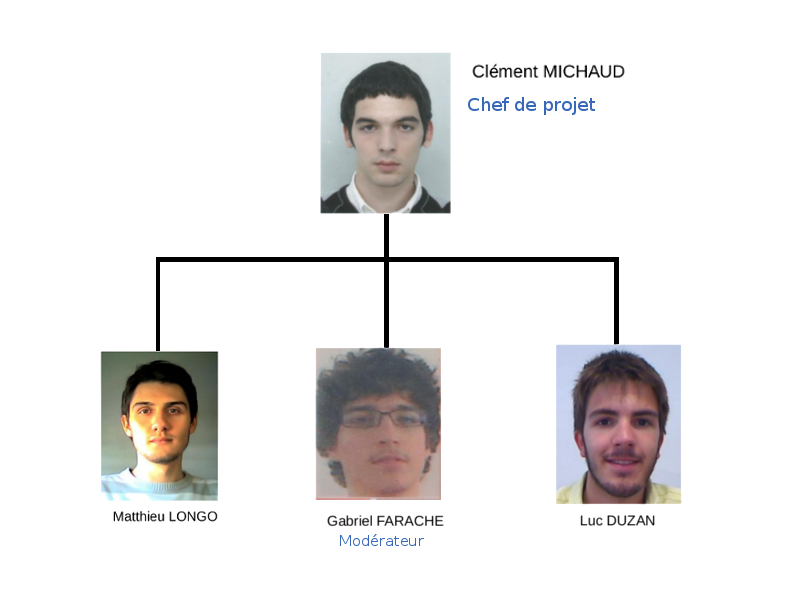
\includegraphics[scale=0.4]{hierarchie.png}
\caption{Hiérarchie de l'équipe}
\label{hierarchie-equipe}
\end{figure}

Ce dernier a été désigné chef de projet par les membres de l'équipe à la fin de la rédaction du projet documentaire. Puis à la suite d'un cours de Conduite de Projet donné par M. HAMADOUCHE, Gabriel FARACHE a été choisi comme modérateur de l'équipe.\\
La recherche documentaire précédent le démarrage du projet a permis de fixer strictement les spécifications techniques et les limites du projet. Le projet a été facile à partitionner grâce à l'existence de trois grands axes de développement parallèles. Cette configuration de projet a permis à l'équipe de créer trois groupes de travail indépendants. Un premier sur du développement logiciel, un deuxième sur du développement matériel en Verilog et un troisième de deux élèves sur la reconfiguration à chaud.\\
Une telle configuration a pu être appliquée au début du développement mais a vite été limitée à cause de la difficulté du sujet. Par la suite, dû aux nombreuses problématiques qui se sont posées, une attitude \textbf{Agile} a été adoptée. Des membres de l'équipe ont été réquisitionnés pour travailler sur un point ou une problématique précise. Cela a permis au groupe de traiter rapidement et efficacement des besoins essentiels nécessaires à l'avancement du reste du projet.